\documentclass{beamer}

\usepackage{graphicx}
\usetheme{Szeged}
\usecolortheme{beaver}

\author{Anne Wanningen \and Xeryus Stokkel}
\title[Week 4]{Introduction to Computer Graphics Raytracer week 5}

\begin{document}

\maketitle

\section{Meshes}

\begin{frame}
	\begin{columns}[T]
		\begin{column}{.45\textwidth}
			\begin{figure}
				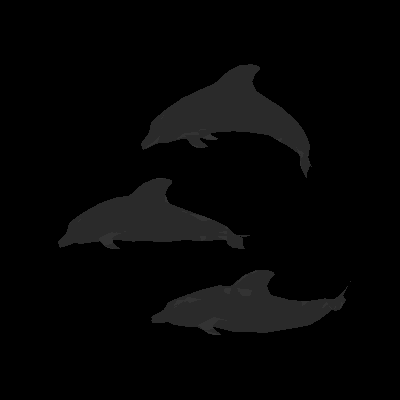
\includegraphics[width=\textwidth]{dolphins-incorrect}
			\end{figure}
		\end{column}
		\begin{column}{.45\textwidth}
			\begin{figure}
				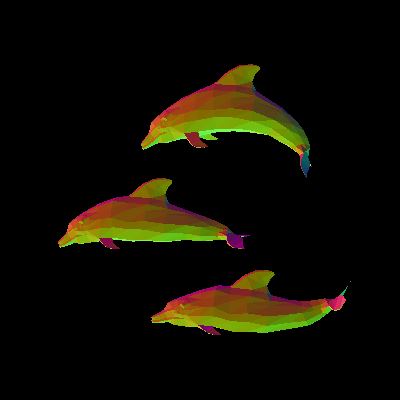
\includegraphics[width=\textwidth]{dolphins-normal-incorrect}
			\end{figure}
		\end{column}
	\end{columns}
\end{frame}

\begin{frame}
	\begin{columns}[T]
		\begin{column}{.45\textwidth}
			\begin{figure}
				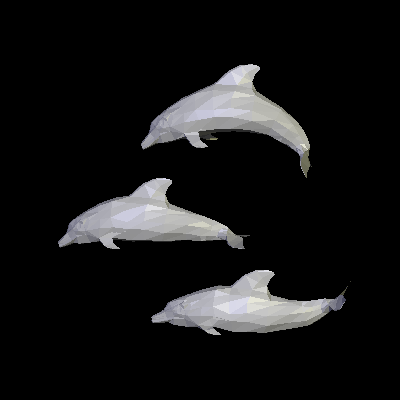
\includegraphics[width=\textwidth]{dolphins-correct}
			\end{figure}
		\end{column}
		\begin{column}{.45\textwidth}
			\begin{figure}
				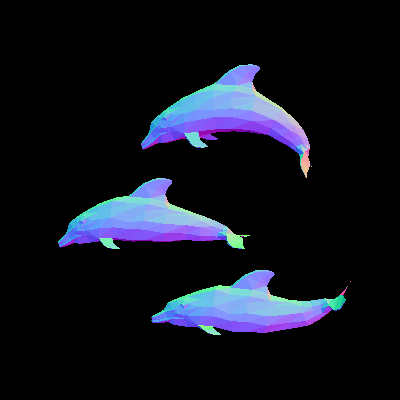
\includegraphics[width=\textwidth]{dolphins-normal-correct}
			\end{figure}
		\end{column}
	\end{columns}
\end{frame}

\begin{frame}
	End results with material colours.
	\begin{columns}[T]
		\begin{column}{.45\textwidth}
			\begin{figure}
				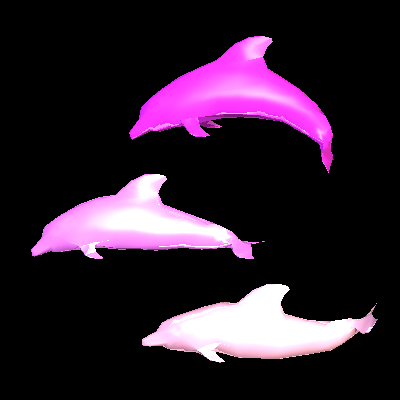
\includegraphics[width=\textwidth]{dolphins2}
			\end{figure}
		\end{column}
		\begin{column}{.45\textwidth}
			\begin{figure}
				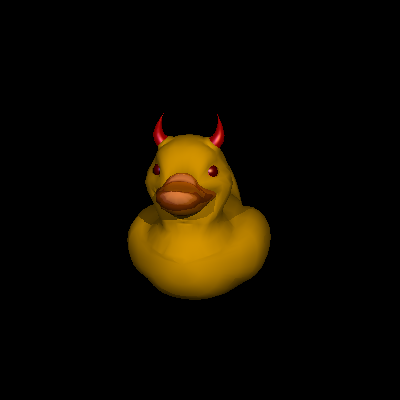
\includegraphics[width=\textwidth]{devilduk}
			\end{figure}
		\end{column}
	\end{columns}
\end{frame}

\section{Gooch shading}
\begin{frame}
	\begin{figure}
		\includegraphics[height=.9\textheight]{raytracer/scene01-gooch}
	\end{figure}
\end{frame}

\end{document}
